 \subsubsection{Overview}


This section is about the SmartAlvarTagDetection Component. The component is used to identify the Alvar Tags on the MPS machines, which is required for the exploration phase where the robots have to explore the game field and find MPS machines and identify the MPS based on their Alvar Tag. \\

Each MPS has their own Alvar Tag, one in the front and one in the back of the machine. This is important for the production phase later. On the field there are seven machines for each team. There are four types of MPS Machines, Base station, Cap station, Ring station and Storage station. All together there are 14 machines with 28 Alvar Tags. \\
Bild von Alvar Tag auf einer MPS. \\

The main idea is that the SmartAlvarTagDetection component identifies the tags. To do so, the component uses an algorithm to determine the Alvar Tag. Therefore, the component needs a picture of the Tag which is taken by a webcam mounted on each of the robotinos and operated by the SmartUnicapImageServer. The SmartAlvarTagDetection components is only one out of many components that are operated and instructed by the InstructionPlanner via the Sequencer (LISPServer). \\
Explain how to operate SmartAlvarTagDetection and SmartUnicapImageServer with DeploymentAlvarTagTest

\subsubsection{CommObjects}

This section describes the CommObjects that are used to communicate with the InstructionPlanner and other componentes.

\subsubsection{Previous State}

The team from the previous semester already had an implementation of the SmartAlvarTagDetection. In their version, they only had implemented the algorithm to scan pictures and identify whether there is a tag or not. They could not communicate with other components or the InstructionPlanner. \\

\begin{figure}[h]
\centering
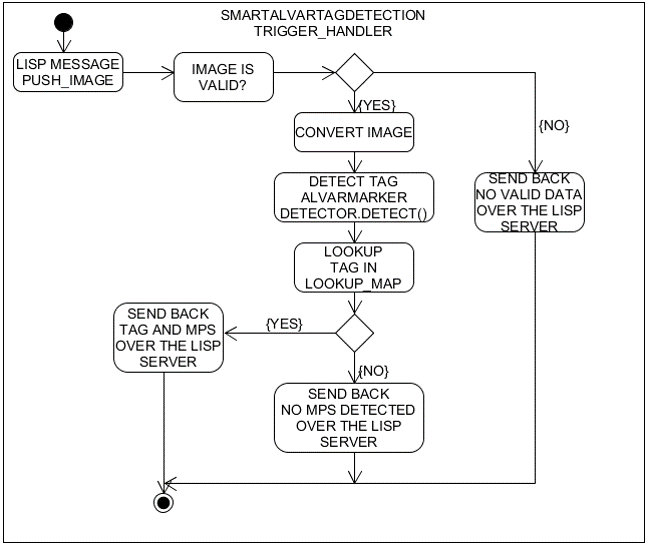
\includegraphics[scale=0.5]{pic/SmartAlvarTagDetectionFlow.png}
\caption{Describes the flow of the SmartAlvarTagDetection Trigger Handler}
\label{fig:smartAlvarFlow}
\end{figure}


At first, the SmartUnicapImageServer is being activated to take a picture and push an image to the SmartAlvarTagDetection. If the SmartUnicapImageServer is done, the LISP Server starts the SmartAlvarTagDetection Trigger Handler. The first thing the Trigger Handler does, is performing a validity check on the picture, to see if the picture can be used or not. If it is not valid, it returns a message saying that the image is not valid. But if it is valid, the image is converted into a greyscale picure, making it easier to recognize the Alvar Tags. Next, the marker detector has to detect an Alvar Tag on the image. It determines the ID by detecting and scanning the tag. In a lookup table this ID is searched and if there is a tag belonging to the ID, then this marker is returned. Markers consist of the type of station, the side and the team color. If the ID cannot be found an error message is returned, otherwise a positive message is returned. \\
Bild von Lookup table \\

The main Problem in this approach was the weak error handling. When for instance no ID could be found on the image and therefore the lookup was not possible, then the entire Robotino crashed. Another problem was that there was no proper communication with the SmartRobotinoInstructionPlanner. When the MPS was detected and found in the lookup table, the positive message was directly sent to the RefBoxServer and not to the SmartRobotinoInstructionPlanner. The communication flow was not transparent. Another problem, not with the implementation but rather with the Alvar and OPENCV libraries, was that it only was possible to deploy the SmartAlvarTagDetection on one computer. Due to difficulties of installing the libraries.



\subsubsection{Current State}

The current version, which was used in the 2017 RoboCup German Open Logistics Leauge in Magdeburg, is able to identify the tags, communicate with the InstructionPlanner via the LISP Server and has some sort of error handling. When the SmartAlvarTagDetection returns the message, that no tag was found, the InstructionPlanner keeps triggering the component five times and if it still sends no tag was found, one can be sure that there really is no tag and it is not a problem with the algorithm or bad picture quality. \\

\begin{figure}[h]
\centering
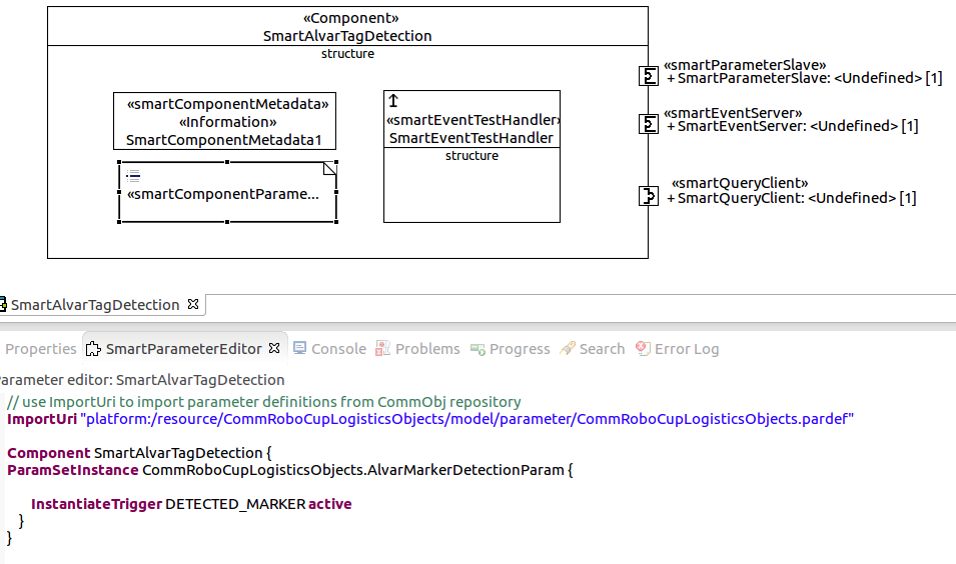
\includegraphics[scale=0.5]{pic/DeploymentAlvarTag.png}
\caption{Shows the model of the SmartAlvarTagDetection component}
\label{fig:smartAlvarFlow}
\end{figure}



The current model consists of a smartEventServer port, a smartQueryClient port and a smartParameterSlave port, but described will be only the first two. The smartEventServer is connected to the LISP Servers' visualMarkerEventClient, which is used to trigger the SmartAlvarTagDetection Trigger Handler.
The other is the SmartQueryClient which is connected to the SmartUnicapImageServers' imageQueryServer to push images that are taken by the webcam to the SmartAlvarTagDetection. The other noticable thing is the smartComponentParameter, which defines the behavior of the SmartAlvarTagDetection component to a Trigger behavior. The smartEventTestHandler is used to check whether an Event fires accordingly. In this case, it tests whether the correct MarkerDetectionState has been set. MarkerDetectionStates are the detected MPS as states. For instance, the tag with ID = 1 has been detected, then the MarkerDetectionState is set to MARKER CYAN CAP STATION 1 FRONT.
